\documentclass{beamer}
\usepackage{graphicx}
\usepackage[english]{babel}
\usepackage{hyperref}
\usepackage{multicol}
\usepackage{amssymb}
\usepackage{amsmath}

\usepackage{xcolor}
\usepackage{tikz}
\usetikzlibrary{calc}


\mode<presentation>
{ 
	\usetheme{Berkeley}
    \usecolortheme{default}
    \usefonttheme{structurebold}
}


% INCLUDE YOUR MENTORS ON YOUR FIRST SLIDE
\title[University of Michigan LoG(M)]{On the Statistics of Character Table of $S_n$}
\author{Tony Zhang, Atharva Kulkarni, Arnav Shah}
\institute{University of Michigan}
\date{Last update \today}

\begin{document}
\begin{frame}
\titlepage
\end{frame}

\begin{frame}{Motivations}
    \begin{definition}
        The character of group element $g \in G$ is, $\chi(g) = Tr(\rho(g))$ where $\rho: G \rightarrow GL_n(\mathbf{C})$ is the group representation \cite{diaconis}
    \end{definition}
    \begin{itemize}
        \item Studying character tables is incredibly useful as the trace of similar matrices is the same, thus the character of an element is invariant under a change of basis
        \item We aim to improve upon existing algorithms to compute higher order character tables of $S_n$ and analyze various statistics of them (eg. if the dimensions of the irreducible representations converges) 
    \end{itemize}
\end{frame}

\begin{frame}
\frametitle{Creating Character Tables using Partitions}
\begin{definition} [{\cite[Defintion 1]{Zhao08youngta}}]
    A \textit{partition} $\lambda$ = ($\lambda_{1}, \dotsc, \lambda_{k}$) of a natural number $n$ is a decreasing sequence $\lambda_{1} \geq \dotsb \geq \lambda_{k}$ of natural numbers that sums to $n$.
    \label{def:partition} 
\end{definition}

\begin{itemize}
    \item Every conjugacy class $\sigma \in S_{n}$ is determined by its cycle type, and the lengths of the cycles in its cycle decomposition give a partition of $n$. Thus, a bijective correspondence exists between partitions of $n$ and conjugacy classes of $S_{n}$. 
    \item For example, take $n=3$. The partitions of $n$ will be $(1,1,1), (2,1),$ and $(3)$. We can map each partition to $\{id\}$, $\{(12), (23), (31)\}$, $\{(123), (132)\}$, respectively.
    \item Similarly, there is a bijective correspondence between partitions of $n$ and irreducible representations of $S_{n}$. For more details, please see \cite{Zhao08youngta}.
\end{itemize}
\end{frame}


\begin{frame}
\frametitle{Creating Character Tables using Partitions (cont.)}
\begin{itemize}
    \item Thus, for every natural number $n$, one can organize the data of all values of irreducible characters on conjugacy classes of $S_{n}$ in a square table, called the character table, with rows and columns indexed by the partitions of $n$. 
    \item The character table of $S_{3}$ can be seen below in table \ref{tab:s3}:
\end{itemize}

\begin{table}[htbp]
    \centering
    \label{tab:s3}
    \begin{tabular}{c|c c c}
        & (1,1,1) & (2,1) & (3) \\
        \hline
        (3) & 1 & 1 & 1 \\
        (2,1) & 2 & 0 & -1 \\
        (1,1,1) & 1 & -1 & 1 \\
    \end{tabular}
    \caption{Character Value Table of S3}
\end{table}
\end{frame}

\begin{frame}
\frametitle{Heatmap of character table for $n=6$}

\begin{figure}[H]
  \centering
  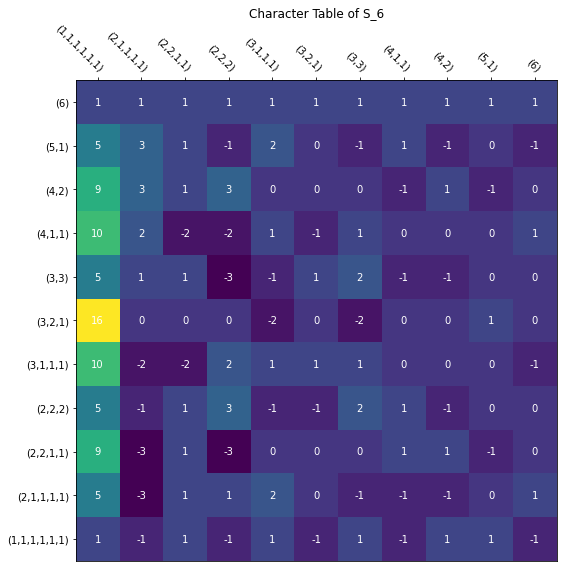
\includegraphics[width=0.4\linewidth]{char_table_6_heatmap.png}
  \caption{Heatmap of Character Table for $n=6$ 
 \footnote{ \tiny See the \href{https://github.com/TonyZhang2004/Character_Table_of_Symmetric_Groups/blob/main/char_table.ipynb}{\textcolor{blue}{program}}}}
  \label{fig:char_6}
\end{figure}

\begin{itemize}
	\item Rows are labeled with partitions corresponding to irreducible representations, columns are labeled with partitions corresponding to conjugacy classes.
\end{itemize}

\end{frame}

\begin{frame}
\frametitle{Frobenius Formula}
\begin{theorem} [Frobenius Formula]
    \begin{itemize}
\item Given an integer partition $\lambda = \lambda_1 + \lambda_2 + \cdots + \lambda_k$ of $n$, let $\chi^{\lambda}$ be the corresponding irreducible character of $S_n$. 
\item Let $\chi^{\lambda}_{\mu}$ be short for the value of $\chi^{\lambda}$ at any $g$ with cycle type $\mu$, denote $l_j  =\lambda_j + k - j$, and $i_j$ the number of times $j$ appears in $\mu$, so $\sum\limits_j i_jj = n$
\item We have the following Frobenius Formula: 

 $\chi^{\lambda}_{\mu} = \text{coeff. of }  x_{1}^{l_1} x_{2}^{l_2}\cdots x_{k}^{l_k}$ in $\Delta(x) P_{\mu}(x)$
 
  
where $\Delta(x) = \prod\limits_{1 \leq i < j \leq k} (x_i-x_j)$, $P_\mu(x) = \prod\limits_j P_j(x_1,\cdots, x_k)^{i_j}$, where $P_j(x_1,\cdots, x_k) = x_1^j + \cdots + x_k^j$ is the $j$-th sum.
\end{itemize}
\end{theorem}
\end{frame}


\begin{frame}
\frametitle{Heatmap of character table for $n=20$}
\begin{figure}[H]
  \centering
  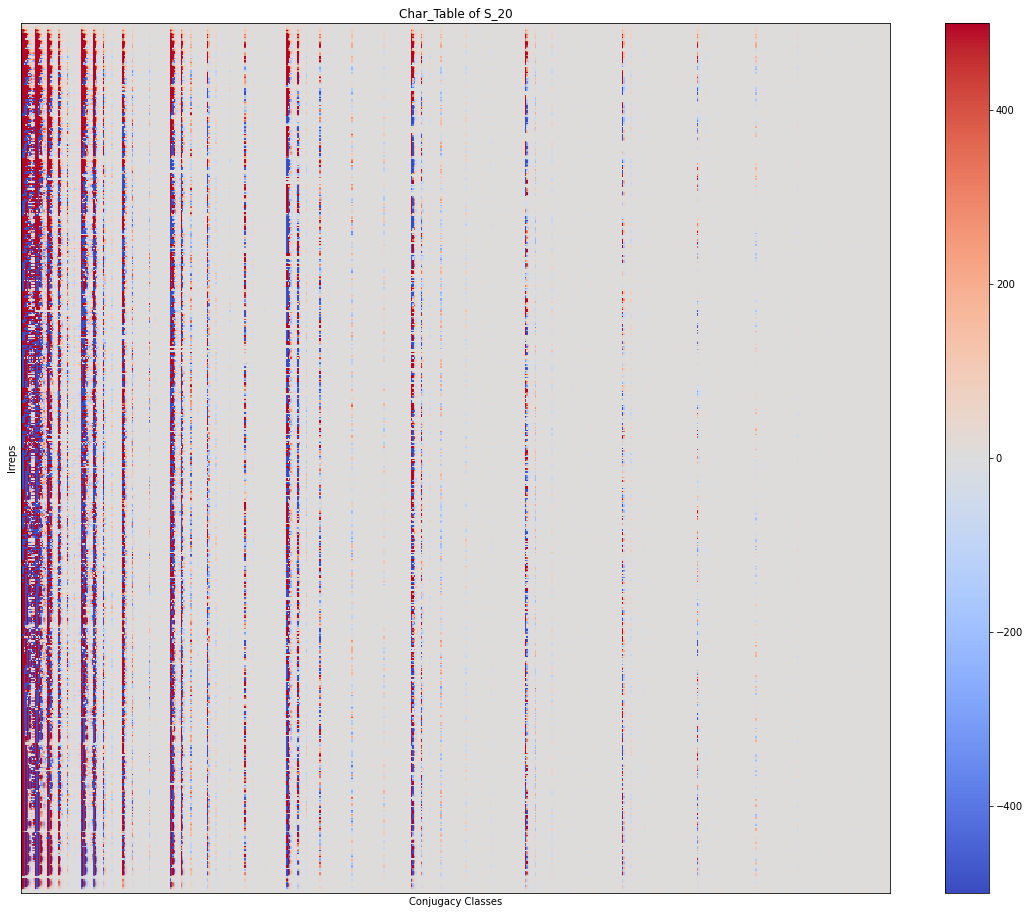
\includegraphics[width=0.6\linewidth]{char_table_20.png}
  \begin{center}
      \caption{\tiny Heatmap of Character Table for $n=20$ (values truncated within $\pm 500$)\footnote{ \tiny See the \href{https://github.com/TonyZhang2004/Character_Table_of_Symmetric_Groups/blob/main/char_table.ipynb}{\textcolor{blue}{program}}}}
  \end{center}
  
  \label{fig:char_20}
\end{figure}
\end{frame}




\begin{frame}
\frametitle{Hooks}
\begin{itemize}
    \item The hook $h$ associated to a box $b$ in the Young diagram of $\lambda$ consists of the box $b$ together with all the boxes directly to its right and directly below it. 
    \item The hook length of $h$, denoted by $l(h)$, is the number of boxes contained in the hook. 
    \item The height of the hook $h$, denoted by $\text{ht}(h)$, is one less than the number of rows in the Young diagram of $\lambda$ that contain a box of $h$. 
    \item  Associated to each hook is a border strip, denoted $\text{bs}(h)$, which is the connected region of boundary boxes of the Young diagram running from the rightmost to the bottom-most box of $h$.
\end{itemize}
\centering
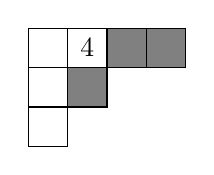
\begin{tikzpicture}[scale=0.5,baseline=(current bounding box.north)]
    \draw (0,3) grid (4,2);
    \draw (0,2) grid (2,1);
    \draw (0,1) grid (1,0);
    \draw[fill=gray] (1,1) rectangle (2,2);
    \draw[fill=gray] (2,2) rectangle (3,3);
    \draw[fill=gray] (3,2) rectangle (4,3);
    % \node at (0.5,0.5) {1};
    % \node at (0.5,1.5) {3};
    % \node at (1.5,1.5) {1};
    % \node at (0.5,2.5) {6};
    \node at (1.5,2.5) {4};
    % \node at (2.5,2.5) {2};
    % \node at (3.5,2.5) {1};
\end{tikzpicture}
\label{fig:younghl}
\end{frame}


\begin{frame}
\frametitle{Murnaghan-Nakayama Rule}
\begin{theorem}[The Murnaghan–Nakayama rule]
Let $n$ and $t$ be positive integers, with $t \leq n$. Let $\sigma \in S_n$ be of the form $\sigma = \tau \cdot \rho$, where $\rho$ is a $t$-cycle, and $\tau$ is a permutation of $S_n$ with support disjoint from $\rho$. Let $\lambda$ be a partition of $n$. Then
\begin{equation*}
    \chi^{\lambda}(\sigma) = \sum_{h \in \lambda, \, \ell(h) = t} (-1)^{\text{ht}(h)} \chi^{\lambda \backslash \text{bs}(h)}(\tau).
\end{equation*}
\end{theorem}

\begin{itemize}
    \item $\chi^{\lambda}(\sigma)$ denotes the value of the character of the irreducible representation of $S_n$ corresponding to the partition $\lambda$, evaluated on the conjugacy class of $\sigma$
    \item $\lambda \backslash \text{bs}(h)$ denotes the partition of $n - t$ obtained by removing the border strip $\text{bs}(h)$ from the Young diagram of $\lambda$
\end{itemize}
\end{frame}



\begin{frame}
\frametitle{Notion of Abacus}
\begin{itemize}
    \item An abacus is a bi-infinite sequence of 0’s and 1’s beginning with an infinite sequence of 1’s and ending with an infinite sequence of 0’s. 
    \item E.g.: \[ \ldots, 1, \ldots, 1, 1, 0, 0, 1, 0, 1, 1, 0, 0, 0, \ldots, 0, \ldots \]
    \item Now, an abacus has a one-to-one correspondence with a partition. 
    \item For a given partition of an integer $n$, we can draw its corresponding Young diagram and trace its border starting from the bottom-left corner to the top-right corner. 
    \item When we move horizontally and vertically, we denote it as a 0 or 1, respectively. This process can be easily reversed as well. 
\end{itemize}
\end{frame}


\begin{frame}
\frametitle{Example}
\begin{itemize}
    \item As an illustration, consider the partition (4,2,1) of 7
    \item Following Figure \ref{fig:youngabaci}, tracing its border as previously mentioned, we move right once, up once, right once, up once, right twice, and lastly up once. 
    \item Our string obtained will be 0,1,0,1,0,0,1 and the corresponding abaci will be: \[ \ldots, 1, \ldots, 1, 1, \textbf{0, 1, 0, 1, 0, 0, 1}, 0, 0, \ldots, 0, \ldots \]
\end{itemize}
\centering
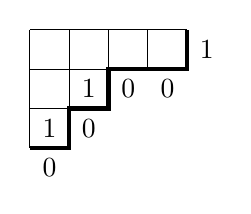
\begin{tikzpicture}[scale=0.5]
    \draw (0,3) grid (4,2);
    \draw (0,2) grid (2,1);
    \draw (0,1) grid (1,0);
    \node at (0.5,-0.5) {0};
    \node at (0.5,0.5) {1};
    \node at (1.5,0.5) {0};
    \node at (1.5,1.5) {1};
    \node at (2.5,1.5) {0};
    \node at (3.5,1.5) {0};
    \node at (4.5,2.5) {1};
    \draw[line width=1.5pt] (0,0) -- (1,0) -- (1,1) -- (2,1) -- (2,2) -- (3,2) -- (4,2) -- (4,3);
\end{tikzpicture}
\label{fig:youngabaci}
\end{frame}


\iffalse
\begin{frame}
\frametitle{References}

\begin{thebibliography}{9}
\setbeamertemplate{bibliography item}[text]
\bibitem{Jane} Jane Doe. {\it A paper with theorems}. Preprint 2018.
\bibitem{logm} Lab of Geometry at Michigan. LoG(M) Beamer Template. {\em University of Michigan Department of Mathematics}. 2018.
\end{thebibliography}

\begin{center}
Special thanks to our mentors, first-names last-names!
\end{center}

\end{frame}
\fi
\begin{frame}{Bibliography}
    \bibliographystyle{plain}
\bibliography{Citations}
\end{frame}

\end{document}

